\section{Detailed control design for agreed plant section}
\label{sec:subsec}

\subsection{Control objectives}

\subsection{Key control loops}

\subsubsection{Reactor R201 temperature control}
\begin{figure}[H]
    \centering
    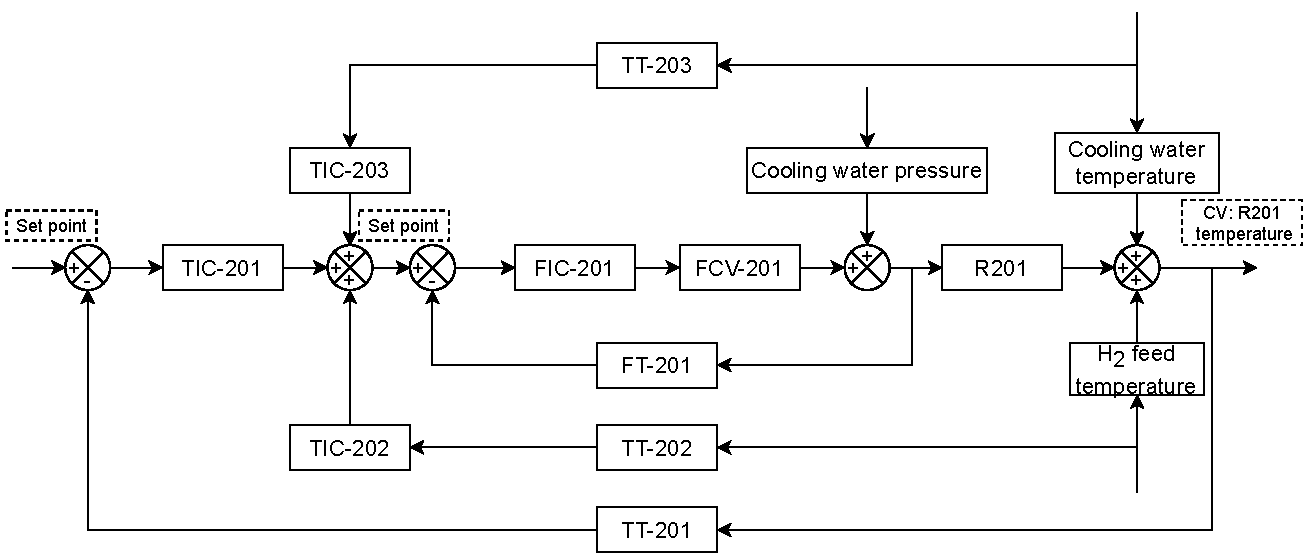
\includegraphics[width=\linewidth]{chapters/4-operation-control/4-Figures/R201-TC.pdf}
    \caption{}
    \label{fig:R201-TC}
\end{figure}

\subsubsection{Reactor R201 pressure control}
\begin{figure}[H]
    \centering
    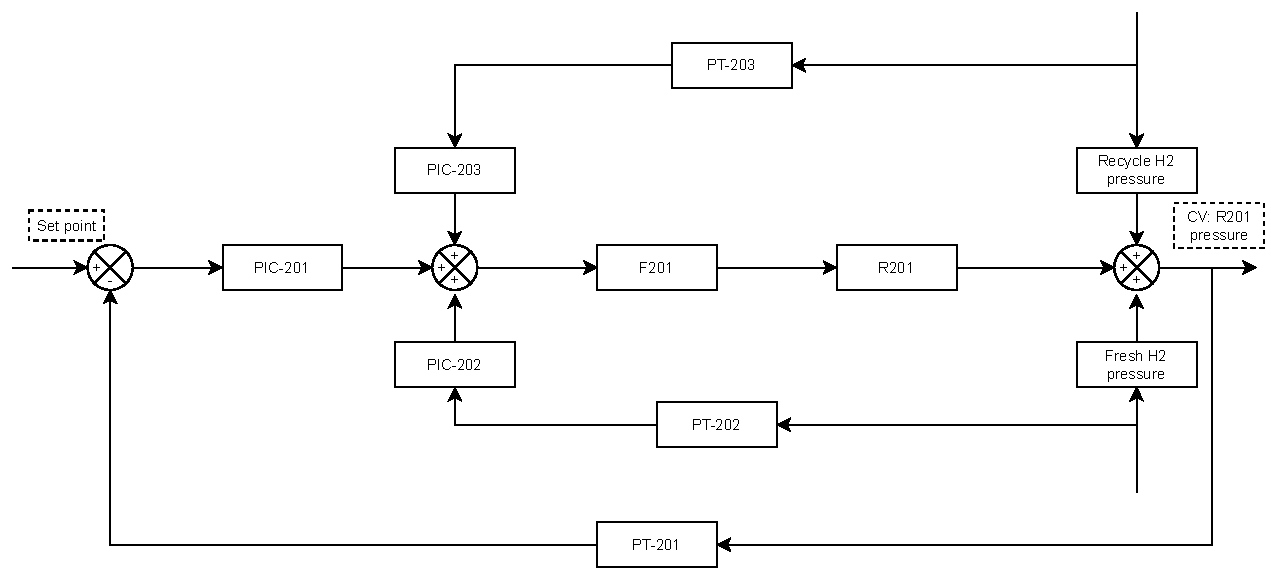
\includegraphics[width=\linewidth]{chapters/4-operation-control/4-Figures/R201-PC.pdf}
    \caption{}
    \label{fig:R201-PC}
\end{figure}

\subsubsection{Reactor R201 level control}
%\begin{figure}[H]
 %   \centering
  %  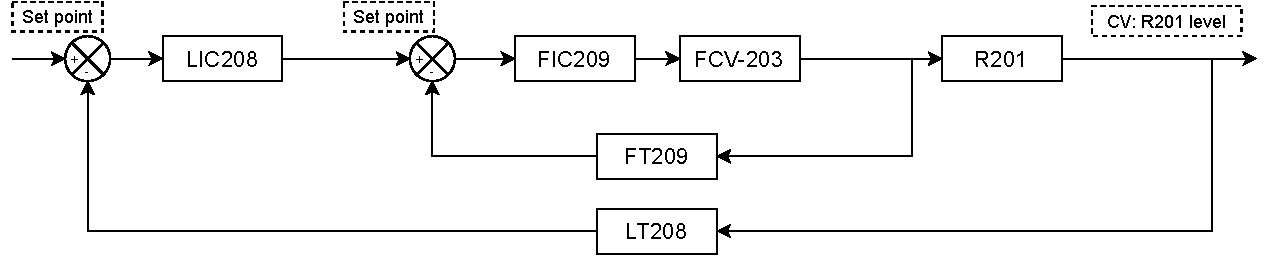
\includegraphics[width=\linewidth]{chapters/4-operation-control/4-Figures/R201-LC.pdf}
   % \caption{}
    %\label{fig:R201-LC}
%\end{figure}

\subsubsection{Reactor feed temperature control}

\subsubsection{Hydrogen recycle control}
\begin{figure}[H]
    \centering
    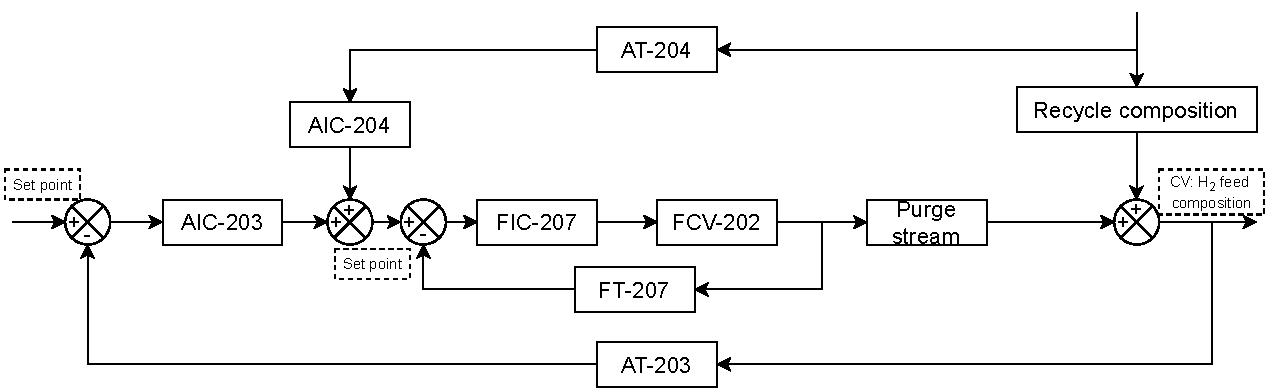
\includegraphics[width=\linewidth]{chapters/4-operation-control/4-Figures/V202-CC.pdf}
    \caption{}
    \label{fig:V202-CC}
\end{figure}

\subsubsection{Reactor outlet flow control}
\begin{figure}[H]
    \centering
    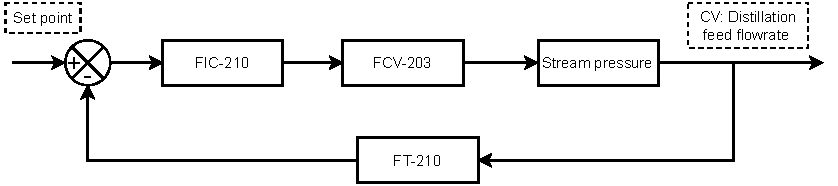
\includegraphics[width=\linewidth]{chapters/4-operation-control/4-Figures/V201-FC.pdf}
    \caption{}
    \label{fig:V201-FC}
\end{figure}


\subsubsection{Control of pressure reduction valve V201}
\begin{figure}[H]
    \centering
    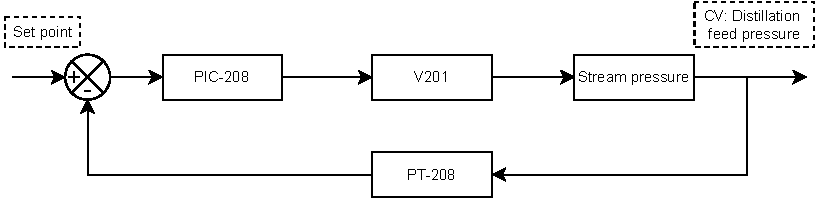
\includegraphics[width=\linewidth]{chapters/4-operation-control/4-Figures/V201-PC.pdf}
    \caption{}
    \label{fig:V201-PC}
\end{figure}

\subsubsection{Distillation column S201 pressure control}
Pressure in distillation columns is regarded as one of the most important parameters to control well, as it not only affects the relative volatilities of the heavy and light keys, but also the shape of the vapour-liquid phase equilibrium curves which determine the compositions of the top and bottoms products of the distillation column. There are several options for for pressure control, such as controlling the vapour flow that is vented from the reflux drum, condenser duty, reboiler duty, recirculation of cooling fluid in the condenser or addition of inerts. Hence the choice of manipulated variable needs to be made carefully considering the relative direct impacts and time delays of each manipulated variable. Controlling the vapour flow that is vented from the reflux drum is the simplest control to implement and usually provides the fastest response as the amount of gas holdup in the column directly affects its pressure. In addition, the amount of vapours in the reflux drum S204 is much larger compared to the condensed liquid flow, so the direct impact of vapour flowrate on column pressure would be large. This avoids a situation where the flow control valve becomes saturated and unable to regulate pressure effectively. 

An optimal feedback control was designed with the vapour flowrate from the reflux drum as the manipulated variable. A pressure transmitter (PT-206) measures the pressure in the column, which is monitored by a pressure controller (PIC-206) that regulates a flow control valve (FCV-205) on the vent stream from the reflux (Figure \ref{fig:S203-PC}.

\begin{figure}[H]
    \centering
    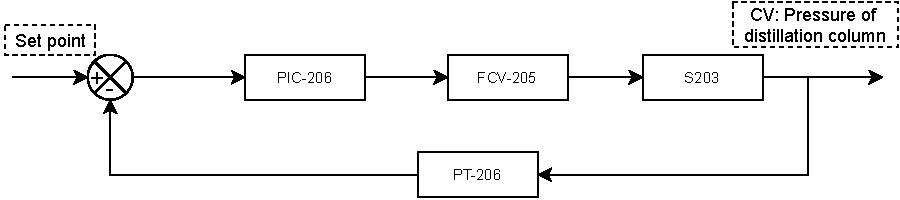
\includegraphics[width=\linewidth]{chapters/4-operation-control/4-Figures/S203-PC.pdf}
    \caption{}
    \label{fig:S203-PC}
\end{figure}

\subsubsection{Bottom stream composition control}
A composition control loop in the distillation column is also necessary to ensure a high recovery of o-toluidine. Since o-toluidine is found in the bottoms stream, reboiler duty was chosen as the manipulated variable in order to reduce the lag time of the controller. A composition analyser (AT-205) measures the concentration of o-toluidine in the bottoms stream and a composition controller (AIC-205) controls the reboiler duty by manipulating a flow control valve on the saturated steam. 

A composition analyser was chosen to allow direct online measurement of the concentration of o-toluidine, 
\begin{figure}[H]
    \centering
    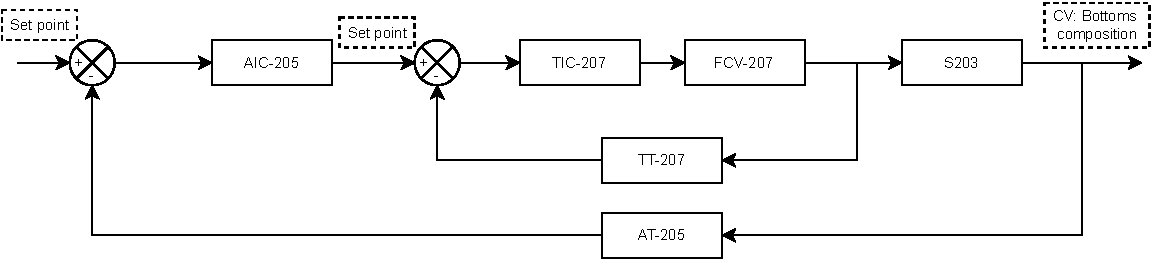
\includegraphics[width=\linewidth]{chapters/4-operation-control/4-Figures/S203-CC.pdf}
    \caption{}
    \label{fig:S203-CC}
\end{figure}


\subsubsection{Distillation column S201 level control}
The level of liquid in the bottom of the distillation column S201 is an important inventory to control in order to prevent the reboiler from drying up and weeping to occur in the column. 
\begin{figure}[H]
    \centering
    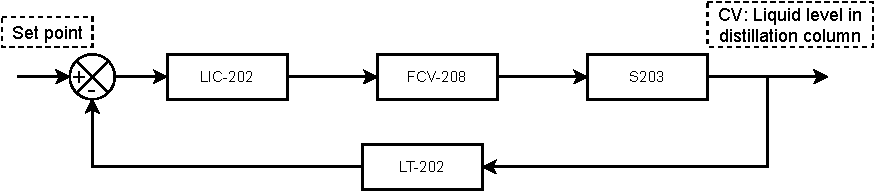
\includegraphics[width=\linewidth]{chapters/4-operation-control/4-Figures/S203-LC.pdf}
    \caption{}
    \label{fig:S203-LC}
\end{figure}

\subsubsection{Reflux drum S204 level control}

\subsubsection{Heat duty of condenser H203 control}
\begin{figure}[H]
    \centering
    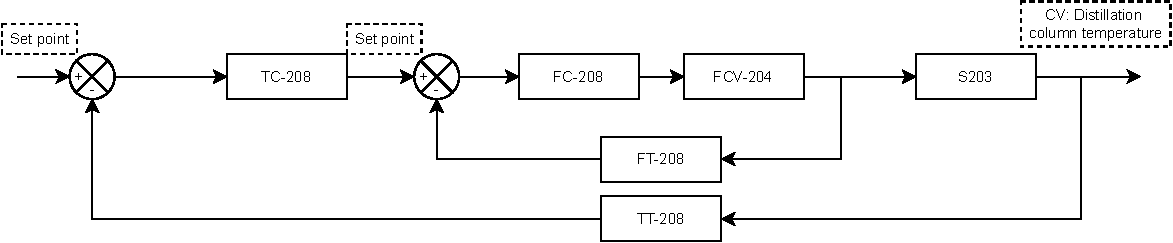
\includegraphics[width=\linewidth]{chapters/4-operation-control/4-Figures/S203C-TC.pdf}
    \caption{}
    \label{fig:S203C-TC}
\end{figure}


\subsubsection{}

\subsection{Safety design}

\subsubsection{Alarms and emergency trips strategy}

\subsubsection{Alarms and safety interlocks design}